
\chapter{Przykładowe zastosowania}

\label{chap:applications}W tym rozdziale przedstawione zostaną przykladowe
zastosowania systemu Bluepath. Na bazie \dcsname{wątków rozproszonych},
\dcsname{pamięci rozproszonej} i nadbudowanych nad nią abstrakcji
listy i słownika przygotowane zostały projekty:
\begin{itemize}
\item \dcsstrong{DLINQ} (ang.~\dcsemph{Distributed Language Integrated Query})
-- dostawca metod manipulacji kolekcji w sposób zgodny z obecnym już
w środowisku .NET dla standardowych, nierozproszonych kolekcji, 
\item \dcsstrong{MapReduce} -- abstrakcja specjalizowana do uruchamiania
zadań w modelu mapowania i redukcji z możliwością zlecania zadań bez
konieczności ponownej kompilacji systemu i dystrybuowania nowej wersji
plików wykonywalnych na węzły,
\item \dcsstrong{System uzupełniania wyrazów} -- system przygotowujący
na podstawie podanej kolekcji dokumentów bazę prefiksów, która jest
wykorzystywana do realizacji systemu podpowiedzi słów na podstawie
pierwszych liter wpisywanych przez użytkownika,
\item \dcsstrong{Obliczanie przybliżenia liczby $\pi$} -- algorytm obliczający
przybliżoną wartość liczby $\pi$, który umożliwił przeprowadzenie
testów porównawczych szybkości obliczeń w klastrze bez wykorzystania
\dcsname{pamięci rozproszonej} w stosunku do obliczeń prowadzonych
na pojedynczym węźle.
\end{itemize}

\section{DLINQ}

Jednym z przykładowych zastosowań biblioteki Bluepath jest Distributed
Language Integrated Query (DLINQ) -- zbiór metod roszerzających możliwości
operowania na kolekcjach bazowanych na \dcsname{pamięci rozproszonej}.
Obecna implementacja służy jako przykład (ang.~\dcsemph{proof of concept})
wykorzystania możliwości dostarczanych przez bibliotekę Bluepath i
dlatego dostarcza implementację podzbioru metod standardowego zestawu
LINQ:
\begin{itemize}
\item \dcscode{Select} -- operacja ta pozwala przetransformować obiekt,
np. wybierając jedynie podzbiór jego atrybutów, lub zmieniając typ
obiektu,
\item \dcscode{SelectMany} -- operacja podobna do \dcscode{Select} z tą
różnicą, że pojedynczy obiekt w wyniku transformacji zmieniany jest
w kolekcję obiektów, a powstałe w ten sposób kolekcje są łączone w
jedną,
\item \dcscode{Where} -- operacja ta pozwala wyfiltrować te obiekty, które
spełniają podany warunek,
\item \dcscode{GroupBy} -- operacja pozwalająca grupować obiekty według
zadanego klucza,
\item \dcscode{Count} -- operacja zliczające obiekty spełniające zadany
warunek. 
\end{itemize}
Operacje te mogą być wykonywane zarówno na dostarczonej z biblioteką
Bluepath liście rozproszonej (opisanej w \ref{sub:----Koncepcja-wspoldzielone-struktury-danych})
jak i na wszystkich obiektach implementujących interfejs \dcscode{IEnumerable}.
W drugim przypadku kolekcja źródłowa zostanie najpierw przetransformowana
do listy rozproszonej, a następnie poddana dalszemu przetwarzaniu.

Sposób wykorzystania rozszerzeń DLINQ jest wzorowany na Parallel Language
Integrated Query (PLINQ). Aby poddać kolekcję przetwarzaniu rozproszonemu
wykonujemy najpierw metodę rozszerzającą \dcscode{AsDistributed}.
Metoda ta posiada jeden obowiązkowy argument -- obiekt zapewniający
dostęp do \dcsname{pamięci rozproszonej}. Następnie na otrzymanym
z tej metody obiekcie można wykonywać operacje zdefiniowane w DLINQ.
Należy jednak mieć na uwadze, że operacje te podlegają założeniom
biblioteki Bluepath i funkcje podawane jako argumenty muszą być funkcjami
statycznymi. Na listingu \ref{lis:Transformacja-kolekcji-DLINQ} przedstawiono
przykładowy kod poddający kolekcję transformacji przy użyciu metody
\dcscode{Select}.

\inputencoding{latin2}\begin{lstlisting}[caption={Transformacja kolekcji przypomocy
metod dostarczonych w DLINQ},label={lis:Transformacja-kolekcji-DLINQ},breaklines=true,language={[Sharp]C},numbers=left]
var inputCollection = new List<double>(100);
...
var processedCollection = (from num in inputCollection.AsDistributed(storage) select Math.Sqrt(num)).ToList();
\end{lstlisting}
\inputencoding{utf8}

W implementacji DLINQ można wyróżnić 3 podstawowe klasy: \dcscode{DistributedQuery},
\dcscode{DistributedEnumerable} oraz \dcscode{UnaryQueryOperator}.
Zostały one dokładniej opisane w poniższych punktach.


\subsection{DistributedQuery}

W celu zapewnienia jednoznacznego rozróżnienia pomiędzy metodami LINQ,
oraz DLINQ wprowadzono klasę \dcscode{DistributedQuery}. Klasa ta
częściowo implementuje interfejs \dcscode{IEnumerable} zapewniając
powiązania pomiędzy metodami tego interfejsu. Stanowi ona bazę z której
wywodzą się wszystkie klasy realizujące poszczególne wywołania DLINQ
(np. \dcscode{Select}) co pozwala na wykonywanie tych samych metod
na instancjach różnych klas składowych DLINQ.


\subsection{DistributedEnumerable}

Statyczna klasa \dcscode{DistributedEnumerable} zawiera wszystkie
metody rozszerzające DLINQ. Każda z tych metod weryfikuje parametry
wejściowe w celu przekazania użytkownikowi zrozumiałych informacji
w przypadku podania błędnych parametrów. Następnie tworzona jest klasa
realizująca wywołanie DLINQ i zwracana użytkownikowi w celu dalszego
przetwarzania (samo wykonanie podobnie jak w LINQ następuje dopiero
wtedy gdy potrzebne są wyniki np. wywołanie metody \dcscode{ToList},
lub enumeracja).

Specjalną metodą rozszerzającą zaimplementowaną w klasie \dcscode{DistributedEnumerable}
jest metoda \dcscode{AsDistributed}. Służy ona przygotowaniu kolekcji
wejściowej do przetwarzania przez metody DLINQ. Jest to realizowane
poprzez opakowanie kolekcji wejściowej klasą \dcscode{DistributedEnumerableWrapper},
która przenosi zawartość kolekcji wejściowej do \dcsname{listy rozproszonej}
(wyjątkiem jest sytuacja, w której kolekcja wejściowa jest \dcsname{listą rozproszoną}).


\subsection{UnaryQueryOperator}

Klasą bazową dla klas implementujących metody DLINQ jest \dcscode{UnaryQueryOperator}.
Jest to klasa, która gromadzi wszystkie metody wspólne dla metod DLINQ
takich jak tworzenie \dcsname{wątków rozproszonych} z wykorzystaniem
ustawień przekazanych przez użytkownika w metodzie \dcscode{AsDistributed},
czy zebranie wyników przetwarzania z poszczególnych \dcsname{wątków rozproszonych}.
Nazwa \dcscode{UnaryQueryOperator} wynika z faktu, że wszystkie metody
DLINQ oparte na tej klasie operują na jednej kolekcji. W przypadku
implementacji metod takich jak \dcscode{Union} -- metoda odpowiadająca
za połączenie dwóch kolekcji -- należałoby stworzyć kolejne klasy,
np. \dcscode{BinaryQueryOperator}.


\section{MapReduce}

\label{sec:applications-MapReduce}W celu porównania pracochłonności
implementacji aplikacji z użyciem bibliteki Bluepath i bez niej przygotowane
zostały aplikacje do realizacji przetwarzania w modelu mapowania i
redukcji zarówno w środowisku Bluepath jak i bezpośrednio z~wykorzystaniem
platformy Windows Communication Foundation~\cite{MSDN:WhatIsWindowsCommunicationFoundation}.
Założeniem aplikacji było, by kod metod \dcscode{Map} i \dcscode{Reduce}
dostarczany był jako kod źródłowy w języku C\# w formie klasy implementującej
odpowiedni interfejs -- \dcscode{IMapProvider} lub \dcscode{IReduceProvider}
-- przedstawiony na listingu \ref{lis:applications-MapReduce-IMapProvider-IReduceProvider}
i składowany razem z danymi w~\dcsname{pamięci rozproszonej}. Kompilacja
kodu miała odbywać się na węzłach bezpośrednio przed wykonaniem metody,
do zrealizowania tego celu wybrana została biblioteka CS-Script~\cite{CS-Script}. 

\noindent %
\begin{minipage}[t]{1\textwidth}%
\inputencoding{latin2}\begin{lstlisting}[caption={Interfejsy
IMapProvider i IReduceProvider},label={lis:applications-MapReduce-IMapProvider-IReduceProvider},breaklines=true,language={[Sharp]C},numbers=left]
public interface IMapProvider 
{
   IEnumerable<KeyValuePair<string, string>> Map(string key, string value); 
}

public interface IReduceProvider 
{
   KeyValuePair<string, string> Reduce(string key, IEnumerable<string> values); 
}
\end{lstlisting}
\inputencoding{utf8}%
\end{minipage}


\subsection{Koordynator}

Główną klasą w aplikacji jest \dcsname{koordynator}, który pełni
rolę nadzorcy zadań (z tego powodu nazywany jest także \dcsemph{JobTrackerem}).
Jego zadaniem jest przydzielanie zdań mapowania i redukcji podległym
węzłom. Poniżej opisano jego implementacje z wykorzystaniem biblioteki
Bluepath jak i w oparciu bezpośrednio o technologię WCF.


\subsubsection*{Koordynator oparty o Bluepath}

W środowisku Bluepath jego zadanie sprowadzało się w pierwszej fazie
przetwarzania do uruchomienia \dcsname{wątków rozproszonych} w
liczbie odpowiadającej liczbe plików wejściowych, które były inicjowane
metodą, która:
\begin{itemize}
\item ładowała kod metody \dcscode{Map} z \dcsname{pamięci rozproszonej}, 
\item wykonywała skompilowany kod \dcsemph{mappera} na wskazanym fragmencie
danych wejściowych z \dcsname{pamięci rozproszonej},
\item zapisywała wygenerowane pary klucz-wartość do \dcsname{pamięci rozproszonej},
\item zwracała listę kluczy jako wynik wykonania \dcsname{wątku rozproszonego}
do \dcsname{koordynatora}.
\end{itemize}
Zainicjowane w ten sposób wątki były następnie uruchamiane z parą
parametrów -- nazwą pliku zawierającego dane do przetworzenia oraz
nazwą pliku z kodem źródłowym metody \dcscode{Map}. W drugiej fazie
przetwarzania tworzonych było tyle rozproszonych wątków, ile kluczy
było wynikiem pierwszej fazy. Każdy z nich inicjowany był metodą,
która:
\begin{itemize}
\item ładowała kod metody \dcscode{Reduce} z \dcsname{pamięci rozproszonej},
\item wykonywała skompilowany kod \dcsemph{reducera} na wskazanym fragmencie
danych wejściowych z \dcsname{pamięci rozproszonej},
\item zapisywała wygenerowane pary klucz-wartość do \dcsname{pamięci rozproszonej},
\item zwracała listę kluczy jako wynik wykonania rozproszonego wątku do
\dcsname{koordynatora}.
\end{itemize}
Przygotowywana jest lista przydziału kluczy do przetwarzania poszczególnym
wątkom dokonującym redukcji, po czym są one uruchamiane z parą parametrów
-- kluczem oraz nazwą pliku z kodem źródłowym metody \dcscode{Reduce}.


\subsubsection*{Koordynator w technologii WCF}

W projekcie bez użycia biblioteki Bluepath koordynator jest opisany
za pomocą interfejsu definiującego kontrakt usługi (\dcscode{ServiceContract})
i udostępnia końcówkę WCF (ang.~\dcsemph{WCF endpoint}). Interfejs
ten został przedstawiony na listingu \ref{lis:applications-MapReduce-ICoordinatorService}.
W tej implementacji koordynator, oprócz zlecania wykonania zadań,
musi również zająć się innymi zadaniami związanymi z obsługą klastra:
\begin{itemize}
\item rejestrowywaniem i wyrejestrowywaniem węzłów, udostępnianiem ich listy
(metody \dcscode{AddWorker}, \dcscode{RemoveWorker}, \dcscode{GetWorkers}),
\item udostępnianiem wyników przetwarzania, zarówno pełnych jak i częściowych,
jeżeli przetwarzanie jeszcze trwa (\dcscode{GetResults}),
\item udostępnianiem interfejsu do manipulacji danymi znajdującymi się w
jego części pamięci -- zapisywanie, usuwanie, pobieranie listy plików,
czyszczenie pamięci (\dcscode{AddToStorage}, \dcscode{RemoveFromStorage},
\dcscode{ListStorageFiles}, \dcscode{CleanStorage}).
\end{itemize}
Pliki, które mają być przetwarzane oraz kod metod Map i Reduce muszą
w pierwszej kolejności trafić do pamięci koordynatora. Poszczególne
pliki są następnie wysyłane do konkretnych węzłów, którym przydzielone
zostało zadanie ich przetwarzania. Podobnie po zakończeniu fazy mapowania
koordynator przygotowuje plan wykonania fazy redukcji i rozsyła w
klastrze listę przydziału kluczy do węzłów. Na tej podstawie węzły
mogą przesłać między sobą wyniki pośrednie. Po zakończeniu przetwarzania
węzły przesyłają pliki wynikowe do pamięci koordynatora.

\inputencoding{latin2}\begin{lstlisting}[caption={Interfejs ICoordinatorService},label={lis:applications-MapReduce-ICoordinatorService},breaklines=true,language={[Sharp]C},numbers=left]
[ServiceContract]
public interface ICoordinatorService
{
    [OperationContract]
    void AddWorker(Uri uri);

    [OperationContract]
    Uri[] GetWorkers();

    [OperationContract]
    void RemoveWorker(Uri uri);

    [OperationContract]
    bool RunJob(int numberOfMappers, int numberOfReducers, Uri mapCodeFile, Uri reduceCodeFile, Uri[] filesToProcess);

    [OperationContract]
    Uri AddToStorage(string fileName, string content);

    [OperationContract]
    Uri[] ListStorageFiles();

    [OperationContract]
    void RemoveFromStorage(Uri uri);

    [OperationContract]
    void CleanStorage();

    [OperationContract]
    MapReduceResult GetResults();
}

[DataContract]
public class MapReduceResult
{
    [DataMember]
    public Tuple<string, string>[] KeysAndValues { get; set; }

    [DataMember]
    public bool IsRunning { get; set; }
}
\end{lstlisting}
\inputencoding{utf8}


\subsection{Pamięć masowa}

Aplikacja ta korzysta z abstrakcji pamięci masowej, którą definiuje
interfejs \dcscode{IMapReduceStorage}. Został on zaprezentowany na
listingu \ref{lis:applications-MapReduce-IMapReduceStorage}. Udostępnia
on dodatkowe operacje, które umożliwiają np. pobieranie listy istniejących
plików czy listy kluczy wygenerowanych w wyniku fazy mapowania. Interfejs
ten jest wspólny dla implementacji z użyciem środowiska Bluepath --
wynikiem jest klasa \dcscode{BluepathStorage} wykorzystująca \dcsname{pamięć rozproszoną}
-- jak i bez niego -- w tym przypadku jest to \dcscode{FileSystemStorage}
bazujący na systemie plików. Klasa \dcscode{FileSystemStorage} przed
zapisaniem pliku na dysk zamienia jego nazwę na reprezentację w kodowaniu
\dcsstrong{Base64}. Mogło więc się zdarzyć, że w naziwe pliku pojawi
się symbol ,,+''. Po zapisaniu tak zakodowanego klucza za pomocą klasy
\dcscode{System.Uri} następowała zamiana znaku ,,+'' na spację, przez
co wartość przestawała być poprawnym ciągiem zgodnym z~kodowaniem
Base64. Jako rozwiązanie tego problemu zastosowano zamianę spacji
z~powrotem na znaki ,,+'' w momencie odczytu klucza z otrzymanego
\dcscode{Uri}.

\inputencoding{latin2}\begin{lstlisting}[caption={Interfejs IMapReduceStorage},label={lis:applications-MapReduce-IMapReduceStorage},breaklines=true,language={[Sharp]C},numbers=left]
public interface IMapReduceStorage
{
    IEnumerable<Uri> ListFiles();
    string Read(string fileName);
    string Read(Uri uri);
    string[] ReadLines(string fileName);
    void Store(string fileName, string value);
    void Store(Uri uri, string value);
    void Clean();
    string GetFileName(Uri uri);
    IEnumerable<string> GetKeys();
    void Remove(Uri uri);
}
\end{lstlisting}
\inputencoding{utf8}


\subsection{Węzeł obliczeniowy w technologii WCF}

Usługa węzła obliczeniowego jest komponentem obecnym jedynie w wersji
aplikacji zbudowanej w oparciu o technologię WCF (środowisko Bluepath
zapewnia możlwiość uruchamiania procesów roboczych na węzłach bez
dodatkowego nakładu pracy ze strony programisty). Usługa ta zarządza
procesami roboczymi na danym węźle oraz pełni rolę pośrednika między
koordynatorem a procesami roboczymi. Węzły mogą komunikować się między
sobą w celu bezpośredniego przesłania plików pomiędzy fazami mapowania
i redukcji. Interfejs usługi umożliwia:
\begin{itemize}
\item utworzenie nowego procesu roboczego (metoda \dcscode{Init}),
\item uruchomienie przetwarzania w ramach jednego z procesów roboczych (\dcscode{Map},
\dcscode{Reduce}),
\item sprawdzenie, czy przetwarzanie w danym procesie roboczym się zakończyło
(\dcscode{TryJoin}),
\item zlecenie przesłania plików między węzłami roboczymi na podstawie listy
przydziału kluczy do węzłów (\dcscode{TransferFiles}),
\item zapisanie pliku w pamięci procesu roboczego (\dcscode{PushFile}),
\item pobranie informacji o obciążeniu węzła (\dcscode{GetPerformanceStatistics})
-- zajętości pamięci operacyjnej, obciążeniu procesora, ilości wolnego
miejsca na dysku.
\end{itemize}
\inputencoding{latin2}\begin{lstlisting}[caption={Interfejs
IRemoteWorkerService},label={lis:applications-MapReduce-IRemoteWorkerService},breaklines=true,language={[Sharp]C},numbers=left]
[ServiceContract]
public interface IRemoteWorkerService
{
    [OperationContract]
    void Init(int workerId);

    [OperationContract]
    void Map(Uri uri, Uri mapFuncUri);

    [OperationContract]
    void Reduce(Uri uri, Uri reduceFuncUri);

    [OperationContract]
    string[] TryJoin(int workerId, Uri callbackUri);

    [OperationContract]
    Uri[] TransferFiles(int workerId, Dictionary<string, Uri> keysAndUris);

    [OperationContract]
    Uri PushFile(int workerId, string fileName, string content);

    [OperationContract]
    PerformanceMonitor.PerformanceStatistics GetPerformanceStatistics();

    Uri EndpointUri { get; }
}
\end{lstlisting}
\inputencoding{utf8}


\subsection{Wyniki eksperymentu}

Implementacja środowiska do przetwarzania w modelu mapowania i redukcji
zajęła 6~dni dwóm programistom, natomiast z wykorzystaniem biblioteki
Bluepath czas ten skrócił się do 2~dni i to przy zaangażowaniu tylko
jednego programisty, a liczba linii kodu została zredukowana z 585
do 194.


\section{System uzupełniania wyrazów}

Wiele aplikacji operujących na dużej ilości danych próbuje wspomóc
swoich użytkowników pozwalając filtrować dane przy pomocy zapytań
tekstowych. Ponieważ formułowanie zapytań podlega często ograniczeniom,
np. konieczności użycia konkretnych słów kluczowych, można stosować
techniki wspomagające użytkownika w~tym działaniu. 

Jedną z takich technik jest system uzupełniania wyrazów (ang.~\dcsemph{autocomplete}).
W trakcie wpisywania zapytania użytkownikowi prezentowana jest lista
zawierająca sugerowane zakończenia wpisywanego wyrazu. W przypadku
gdy wyraz, który użytkownik miał zamiar wpisać, znajduje się na liście
może on zostać wybrany. W~przeciwnym wpadku użytkownik musi kontynuować
wpisywanie wyrazu.

System tego typu można zrealizować poprzez porównanie wprowadzonego
słowa ze słowami występującymi w przetwarzanych danych. Ponieważ przetwarzanie
wszystkich posiadanych danych w czasie rzeczywistym byłoby bardzo
powolne, można je poddać wstępnej obróbce~--~np. wygenerowaniu i
powiązaniu prefiksów z ich możliwymi rozwinięciami.

System uzupełniania wyrazów został zaimplementowany jako przykład
zastosowania biblioteki \dcsname{Bluepath}. Przetwarzanie zostało
podzielone na trzy odrębne części:
\begin{itemize}
\item wczytywanie danych~--~wytworzenie i powiązanie prefiksów i ich rozwinięć
-- opisane w \ref{sub:zastosowania-autocomplete-Wczytywanie-danych},
\item uzupełnianie wyrazów~--~demonstracja realizacji funkcji podpowiadania
możliwych zakończeń prefiksu -- opisane w \ref{sub:zastosowania-autocomplete-Uzupe=000142nianie-wyraz=0000F3w},
\item czyszczenie stanu systemu~--~przywrócenie całego systemu do stanu
początkowego bez konieczności ponownego uruchamiania aplikacji.
\end{itemize}
Na podział ten miały wpływ dwa czynniki:
\begin{itemize}
\item z założenia przygotowywanie prefiksów (wraz z rozwinięciami) miało
być czynnością niezależną od wyszukiwania możliwych rozwinięć wpisanego
wyrazu~--~system udziela odpowiedzi na podstawie najświeższych posiadanych
danych,
\item w trakcie pisania systemu okazało się, że przydatna jest metoda przywracająca
system do stanu początkowego, a niebędąca częścią głównego przetwarzania.
\end{itemize}

\subsection{Wczytywanie danych}

\label{sub:zastosowania-autocomplete-Wczytywanie-danych}Zaimplementowany
system uzupełniania wyrazów, przed rozpoczęciem wyszukiwania możliwych
zakończeń zadanego prefiksu, musi zostać zainicjalizowany. Dokumenty
zawierające przykładowe słowa są wczytywane przez węzeł inicjalizujący
operację wczytywania danych i dodawane jako elementy \dcsname{listy rozproszonej}.
Następnie każdy \dcsname{wątek rozproszony} pobiera nieprzetworzony
fragment listy i na podstawie zawartych w nim dokumentów uzupełnia
słownik prefiksów i możliwych dla nich uzupełnień. Gdy na liście nie
ma już elementów do przetworzenia, \dcsname{wątek rozproszony} kończy
przetwarzanie. Gdy wszystkie \dcsname{wątki rozproszone} zakończą
przetwarzanie, każdy z węzłów zawiera częściową informację dotyczącą
prefiksów i ich uzupełnień. Fragment funkcji \dcscode{LoadDocuments}
odpowiedzialnej za operację wczytywania danych wykonywaną przez \dcsname{wątek rozproszony}
został przedstawiony na listingu \ref{lis:Fragment-funkcji-LoadDocuments}.

\inputencoding{latin2}\begin{lstlisting}[caption={Fragment funkcji LoadDocuments},label={lis:Fragment-funkcji-LoadDocuments},breaklines=true,language={[Sharp]C},numbers=left]
private static int LoadDocuments(string inputKey, string counterKey, int chunkSize, IBluepathCommunicationFramework bluepath)        
{
	var inputList = new DistributedList<string>(bluepath.Storage as IExtendedStorage, inputKey);
	var inputCount = inputList.Count;
	var counter = new DistributedCounter(bluepath.Storage as IExtendedStorage, counterKey);
	int indexEnd = 0;
	do
	{
		int noOfElements = chunkSize; 
		int indexStart = counter.GetAndIncrease(chunkSize); 
		[...]
		var inputDocuments = new string[noOfElements];    
		inputList.CopyPartTo(indexStart, noOfElements, inputDocuments); 
		foreach (var document in inputDocuments)     
		{               
			var words = document.Split(' ');    
			foreach (var word in words)   
			{                     
				[...] // wygenerowanie prefiks�w i zapisanie ich w pami�ci lokalnej                  
			}                 
		}
	} while (indexEnd <= inputCount);

	return 0;     
}
\end{lstlisting}
\inputencoding{utf8}


\subsection{Uzupełnianie wyrazów\label{sub:zastosowania-autocomplete-Uzupe=000142nianie-wyraz=0000F3w}}

Głównym celem systemu uzupełniania wyrazów jest wyszukiwania możliwych
zakończeń zadanego prefiksu. W tym celu należy przeszukać informacje
posiadane przez każdy z węzłów, a następnie zagregować uzyskane wyniki
częściowe. Aby mieć pewność, że każdy węzeł zostanie przeszukany zastosowano
planistę szeregującego zadania za pomocą algorytmu karuzelowego (opisanego
w punkcie \ref{sub:Implementacja-Szeregowanie-karuzelowy}) i uruchomiono
tyle \dcsname{wątków rozproszonych}, ile znajduje się węzłów w
systemie. Inicjalizacja planisty została przedstawiona na listingu
\ref{lis:zastosowania-autocomplete-Inicjalizacja-planisty-szereguj=000105}.
\inputencoding{latin2}\begin{lstlisting}[caption={Inicjalizacja
planisty szereguj�cego zadania za pomoc� algorytmu karuzelowego},label={lis:zastosowania-autocomplete-Inicjalizacja-planisty-szereguj=000105},breaklines=true,language={[Sharp]C},numbers=left]
var services = connectionManager.RemoteServices.Select(s => s.Key).ToArray();
var scheduler = new RoundRobinLocalScheduler(services);
\end{lstlisting}
\inputencoding{utf8}

Po zakończeniu przetwarzania przez wszystkie wątki należy zagregować
dane. Częścią tej operacji, oprócz połączenia wyników, jest usunięcie
duplikatów, które mogą się pojawić ze względu na to, że w tej implementacji
każdy \dcsname{wątek rozproszony} wykonuje przetwarzanie lokalnie
(niezależnie od pozostałych wątków). Na listingu \ref{lis:zastosowania-autocomplete-Zebranie-wynik=0000F3w-w}
przedstawiono zbieranie wyników oraz usunięcie duplikatów.\inputencoding{latin2}
\begin{lstlisting}[caption={Zebranie
wynik�w w systemie uzupe�niania wyraz�w},label={lis:zastosowania-autocomplete-Zebranie-wynik=0000F3w-w},breaklines=true,language={[Sharp]C},numbers=left]
var joinedResult = new List<string>();
foreach (var thread in threads)
{
	thread.Join();
	joinedResult.AddRange(thread.Result as string[]);
}

var endResult = joinedResult.Distinct().ToArray();
\end{lstlisting}
\inputencoding{utf8}


\section{Obliczanie przybliżenia liczby $\pi$}

\label{sec:Przykladowe-zastosowania-liczba-pi}Metoda Monte Carlo
jest formą symulacji z wykorzystaniem generatora liczb pseudolosowych.
Każde kolejne uruchomienie algorytmu daje nieco inne wyniki, o ile
nie zapewnimy generatorowi takich samych warunków początkowych (ang.~\dcsemph{seed}).
Obliczenie przybliżenia liczby $\pi$ sprowadza się do losowania $n$
razy pary liczb $(x,\thinspace y)$ z~przedziału $[0,\thinspace1]$
i inkrementowaniu licznika $m$, gdy para spełnia warunek $x^{2}+y^{2}\leq1$.
W przykładowej symulacji dla $n=1000000$ otrzymano $m=785930$. Oznacza
to, że $m$ z $n$ sprawdzonych punków znalazło się w obszarze reprezentującym
$\frac{1}{4}$ powierzchni koła, którego środek znajduje się w punkcie
(0, 0) -- patrz rysunek \ref{fig:applications-Monte-Carlo-Pi}. Ostateczne
wyliczenie otrzymanego przybliżenia liczby $\pi$ przedstawia równanie
\ref{eq:applications-Monte-Carlo-Pi}. 
\begin{equation}
p=\frac{m}{n}=\frac{785930}{1000000},\thinspace\thinspace\thinspace p\times4=3,14372\approx\pi\label{eq:applications-Monte-Carlo-Pi}
\end{equation}


\begin{center}
\begin{figure}
\centering{}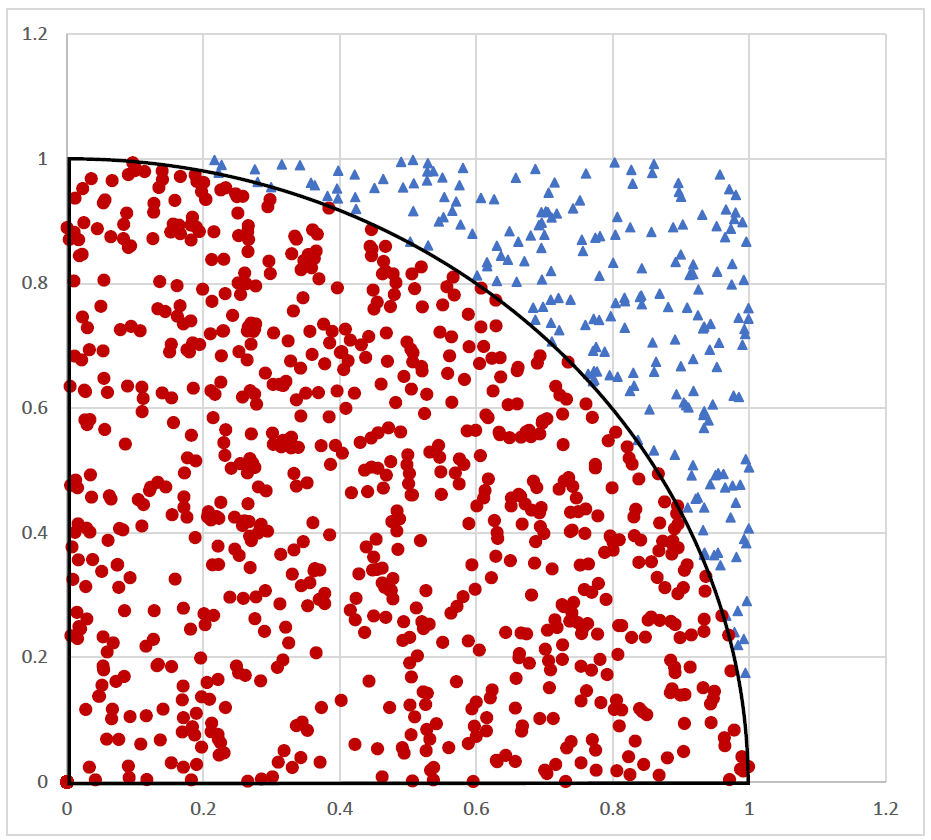
\includegraphics[scale=0.4]{images/monte-carlo-pi}\protect\caption{\label{fig:applications-Monte-Carlo-Pi}Ilustracja obliczania przybliżenia
liczby $\pi$ metodą Monte Carlo}
\end{figure}

\par\end{center}

Zwiększanie liczby próbek $n$ nie musi poprawiać dokładności otrzymanego
wyniku. W zależności od jakości zastosowanego generatora liczb pseudolosowych,
może on w pewnym momencie zakończyć bieżącą sekwencję i rozpocząć
zwracanie liczb z tej samej sekwencji od początku. Ponieważ celem
tego testu nie jest zbadanie dokładności przybliżenia liczby $\pi$
a porównanie szybkości obliczeń w klastrze i na pojedynczym węźle,
jako generator została wybrana klasa \dcscode{System.Random}%
\footnote{%
\begin{minipage}[t]{1\columnwidth}%
Implementacja klasy \dcscode{System.Random} w .NET Framework 4.0
posiada kilka cech, które sprawiają, że nie nadaje się ona do zastosowań,
w których oczekujemy ciągu o wysokim stopniu losowości. 
\begin{itemize}
\item Inicjowanie generatora przez domyślny konstruktor używa aktualnego
czasu. Z tego powodu utworzenie wielu jego instancji w krótkim czasie,
np. w środowisku wielowątkowym, może prowadzić do otrzymania takich
samych sekwencji liczb. Co więcej, przestrzeń inicujująca generator
jest stosunkowo mała -- mając już $2^{16}$ instancji generatora zainicjowanego
losowymi wartościami istnieje duże prawdopodobieństwo otrzymania tej
samej sekwencji wielokrotnie.
\item Dla niektórych wartości parametrów metoda \dcscode{Next} zwraca sekwencje,
których rozkład nie jest równomierny. 
\end{itemize}
W zastosowaniach, w których wymagane jest bezpieczeństwo zaleca się
stosowanie implementacji opartych o metody kryptograficzne, np. \dcscode{System.Security.Cryptography.RNGCryptoServiceProvider}.%
\end{minipage}%
}.

Otrzymane wyniki i ich analiza zostały przedstawione w rozdziale \dcsemph{Testy wydajnościowe i jakościowe}
w punkcie \ref{sub:performance-Obliczanie-przyblizenia-Pi}.
